
\documentclass[border=10pt, 12pt]{standalone}
\usepackage[svgnames]{xcolor}
\usepackage{amsmath}
\usepackage{pgfplots}
\pgfplotsset{compat=newest}
\usepackage[sfdefault]{FiraSans}
\usepackage{FiraMono}
\renewcommand*\familydefault{\sfdefault}
\begin{document}
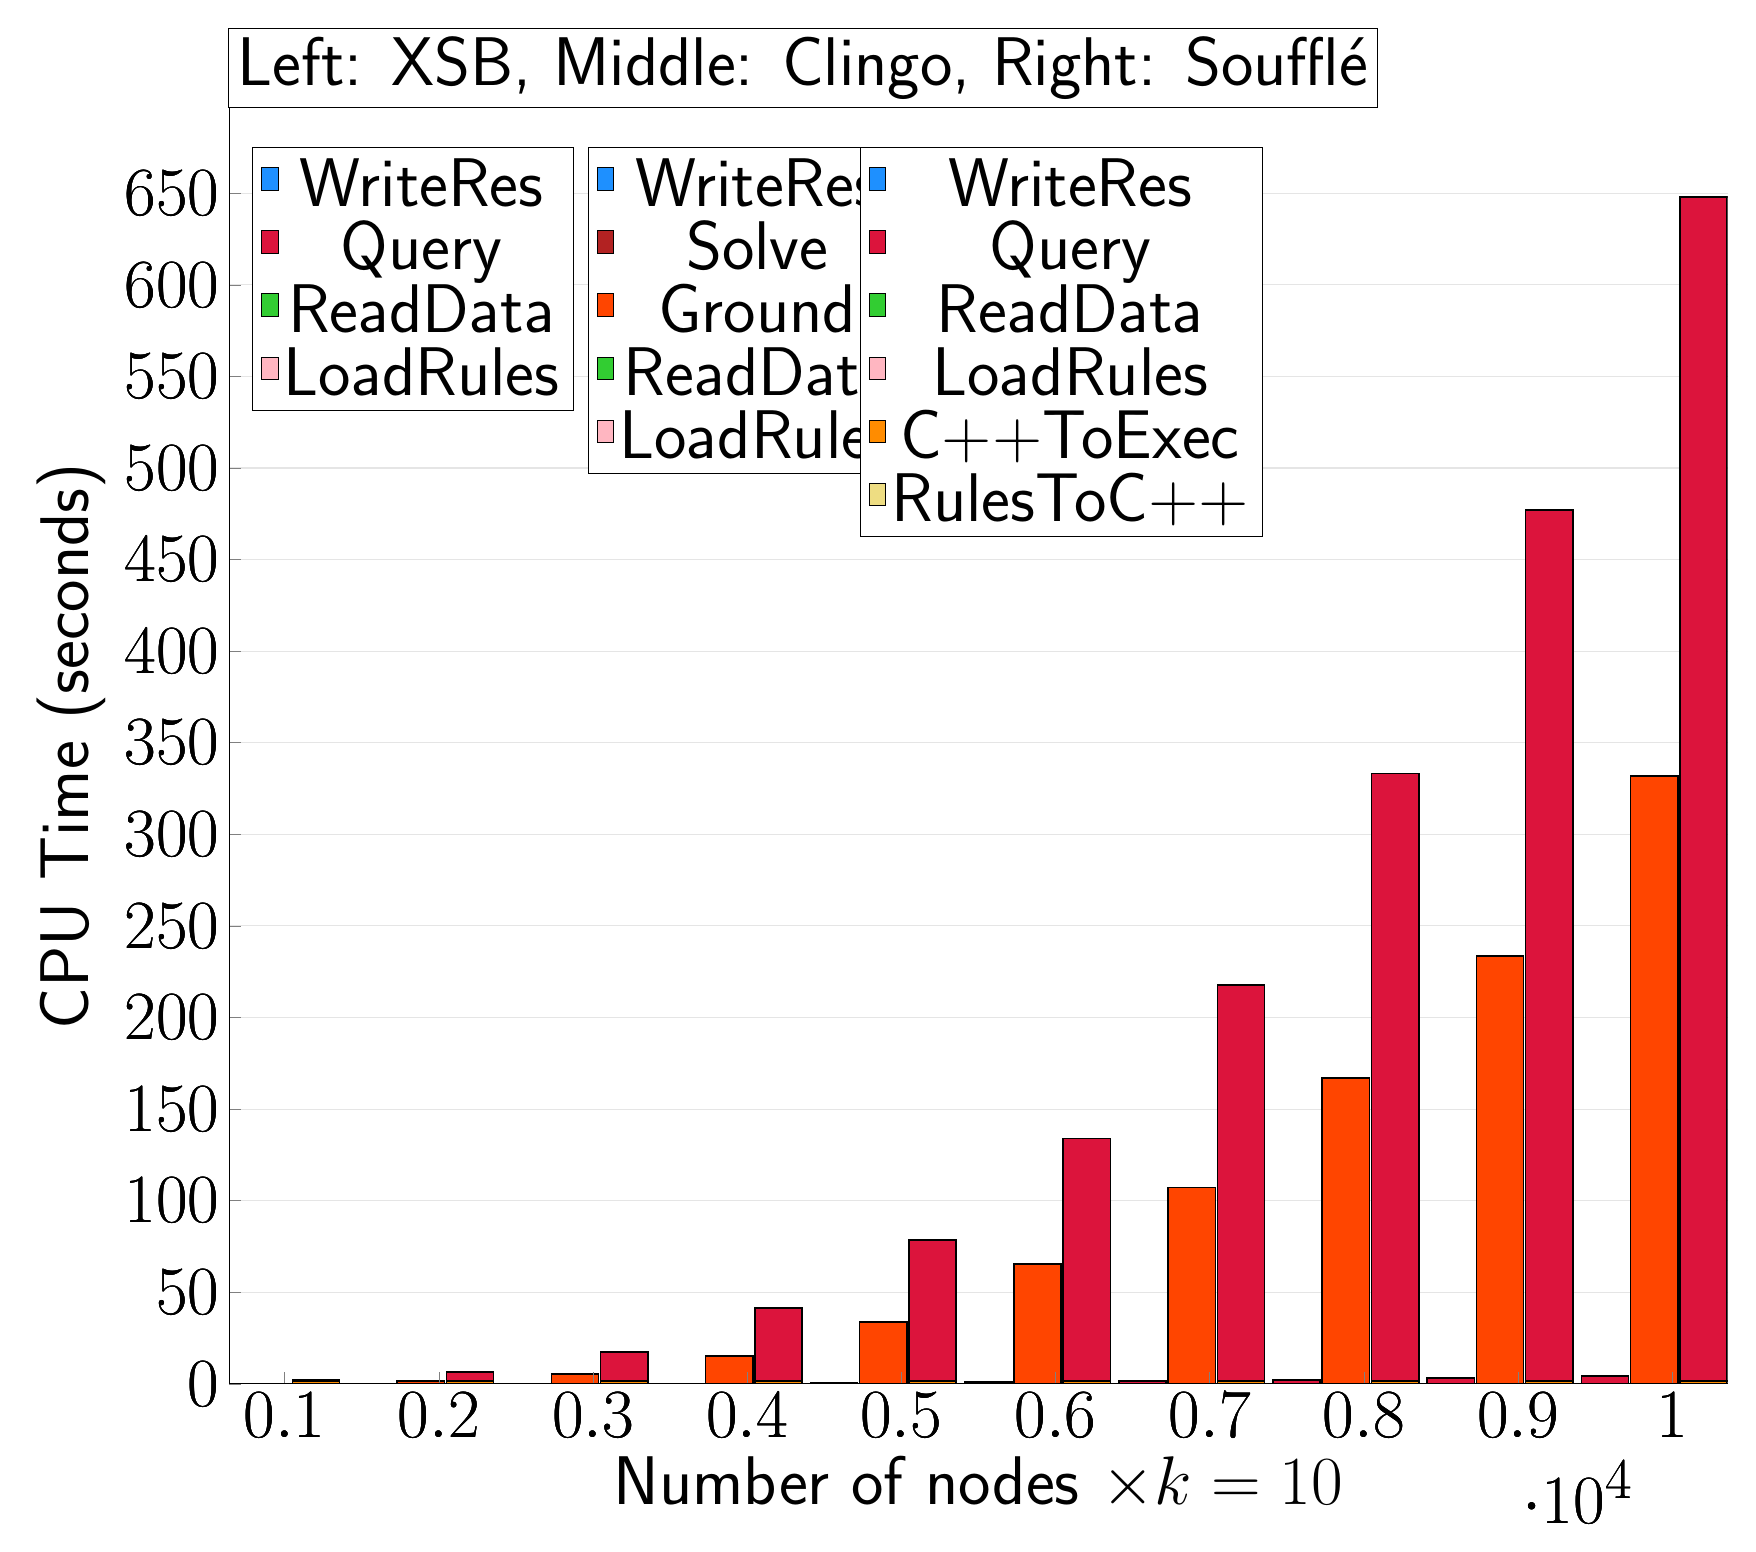
\begin{tikzpicture}
                        \begin{axis}[bar shift=-24.3pt, 
   ybar stacked,
   width=1.7\textwidth,
   bar width=0.6cm,
   ymajorgrids, tick align=inside,
   major grid style={draw=gray!20},
   xtick=data,
   ymin=0, ymax=696.3414,
   axis x line*=bottom,
   axis y line*=left,
   enlarge x limits=0.04,
   legend style={
       at={(0.23, 0.97)},
       anchor=north east,
       legend columns=1,
       font=\Huge,
   },
   ylabel={CPU Time (seconds)},
   xlabel={Number of nodes $\times k=10$},
   label style={font=\Huge},
   tick label style={font=\Huge},
]
\addlegendimage{fill=DodgerBlue, draw=black, line width=0.2pt}
\addlegendentry{WriteRes}
\addlegendimage{fill=Crimson, draw=black, line width=0.2pt}
\addlegendentry{Query}
\addlegendimage{fill=LimeGreen, draw=black, line width=0.2pt}
\addlegendentry{ReadData}
\addlegendimage{fill=LightPink, draw=black, line width=0.2pt}
\addlegendentry{LoadRules}
\addplot +[fill=LightPink, draw=black, line width=0.55pt] coordinates {
(1000, 0.0005522000000000001)
(2000, 0.0005570000000000002)
(3000, 0.0005507999999999996)
(4000, 0.000556)
(5000, 0.0005533999999999994)
(6000, 0.0005547999999999995)
(7000, 0.0005493999999999996)
(8000, 0.0005641999999999993)
(9000, 0.0005514)
(10000, 0.0005507999999999996)
};
\addplot +[fill=LimeGreen, draw=black, line width=0.55pt] coordinates {
(1000, 0.0008961999999999996)
(2000, 0.0017135999999999998)
(3000, 0.0025551999999999997)
(4000, 0.0033902000000000003)
(5000, 0.0042128)
(6000, 0.005051600000000001)
(7000, 0.0058554)
(8000, 0.006689199999999999)
(9000, 0.007532)
(10000, 0.0083348)
};
\addplot +[fill=Crimson, draw=black, line width=0.55pt] coordinates {
(1000, 0.0044354)
(2000, 0.0348032)
(3000, 0.11691320000000001)
(4000, 0.2731402)
(5000, 0.5313167999999999)
(6000, 0.9284899999999998)
(7000, 1.4612399999999999)
(8000, 2.1354846)
(9000, 3.0521022)
(10000, 4.1459534)
};
\addplot +[fill=DodgerBlue, draw=black, line width=0.55pt] coordinates {
(1000, 1.4199999999999803e-05)
(2000, -0.00023919999999999635)
(3000, 0.0011550000000000004)
(4000, -0.0006465999999999861)
(5000, -0.007748200000000027)
(6000, -0.02270739999999998)
(7000, -0.007739399999999996)
(8000, -0.020639199999999924)
(9000, -0.026503400000000087)
(10000, -0.04045659999999973)
};
\end{axis}

\begin{axis}[bar shift=-6.5pt, 
   ybar stacked,
   width=1.7\textwidth,
   bar width=0.6cm,
   ymajorgrids, tick align=inside,
   major grid style={draw=none},
   xtick=data,
   ymin=0, ymax=696.3414,
   axis x line*=none,
   axis y line*=none,
   enlarge x limits=0.04,
   legend style={
       at={(0.454, 0.97)},
       anchor=north east,
       legend columns=1,
       font=\Huge,
   },
   label style={font=\Huge},
   tick label style={font=\Huge},
]
\addlegendimage{fill=DodgerBlue, draw=black, line width=0.2pt}
\addlegendentry{WriteRes}
\addlegendimage{fill=FireBrick, draw=black, line width=0.2pt}
\addlegendentry{Solve}
\addlegendimage{fill=OrangeRed, draw=black, line width=0.2pt}
\addlegendentry{Ground}
\addlegendimage{fill=LimeGreen, draw=black, line width=0.2pt}
\addlegendentry{ReadData}
\addlegendimage{fill=LightPink, draw=black, line width=0.2pt}
\addlegendentry{LoadRules}
\addplot +[fill=LightPink, draw=black, line width=0.55pt] coordinates {
(1000, 0.0)
(2000, 0.0)
(3000, 0.0)
(4000, 0.0)
(5000, 0.0)
(6000, 0.0)
(7000, 0.0)
(8000, 0.0)
(9000, 0.0)
(10000, 0.0)
};
\addplot +[fill=LimeGreen, draw=black, line width=0.55pt] coordinates {
(1000, 0.0)
(2000, 0.0)
(3000, 0.008000000000000007)
(4000, 0.010000000000000009)
(5000, 0.010000000000000009)
(6000, 0.010000000000000009)
(7000, 0.010000000000000009)
(8000, 0.018000000000000016)
(9000, 0.022000000000000013)
(10000, 0.020000000000000018)
};
\addplot +[fill=OrangeRed, draw=black, line width=0.55pt] coordinates {
(1000, 0.182)
(2000, 1.4540000000000002)
(3000, 5.376)
(4000, 15.148000000000001)
(5000, 33.68)
(6000, 65.44800000000001)
(7000, 107.21)
(8000, 167.01600000000002)
(9000, 233.62800000000001)
(10000, 331.832)
};
\addplot +[fill=FireBrick, draw=black, line width=0.55pt] coordinates {
(1000, 0.0)
(2000, 0.0)
(3000, 0.002000000000000135)
(4000, 0.00799999999999983)
(5000, 0.00600000000000307)
(6000, 0.008000000000001251)
(7000, 0.013999999999995794)
(8000, 0.01599999999998545)
(9000, 0.02199999999999136)
(10000, 0.029999999999995454)
};
\addplot +[fill=DodgerBlue, draw=black, line width=0.55pt] coordinates {
(1000, 0.0)
(2000, 0.0)
(3000, -1.3461454173580022e-16)
(4000, -0.00799999999999983)
(5000, -0.00600000000000307)
(6000, -0.006000000000000227)
(7000, -0.01199999999999477)
(8000, -0.01599999999998545)
(9000, -0.02199999999999136)
(10000, -0.029999999999995454)
};
\end{axis}

\begin{axis}[bar shift=11.3pt, 
   ybar stacked,
   width=1.7\textwidth,
   bar width=0.6cm,
   ymajorgrids, tick align=inside,
   major grid style={draw=none},
   xtick=data,
   ymin=0, ymax=696.3414,
   axis x line*=none,
   axis y line*=none,
   enlarge x limits=0.04,
   legend style={
       at={(0.69, 0.97)},
       anchor=north east,
       legend columns=1,
       font=\Huge,
   },
   label style={font=\Huge},
   tick label style={font=\Huge},
]
\addlegendimage{fill=DodgerBlue, draw=black, line width=0.2pt}
\addlegendentry{WriteRes}
\addlegendimage{fill=Crimson, draw=black, line width=0.2pt}
\addlegendentry{Query}
\addlegendimage{fill=LimeGreen, draw=black, line width=0.2pt}
\addlegendentry{ReadData}
\addlegendimage{fill=LightPink, draw=black, line width=0.2pt}
\addlegendentry{LoadRules}
\addlegendimage{fill=DarkOrange, draw=black, line width=0.2pt}
\addlegendentry{C++ToExec}
\addlegendimage{fill=LightGoldenrod, draw=black, line width=0.2pt}
\addlegendentry{RulesToC++}
\addplot +[fill=LightGoldenrod, draw=black, line width=0.55pt] coordinates {
(1000, 0.008000000000000002)
(2000, 0.010000000000000002)
(3000, 0.010000000000000002)
(4000, 0.006000000000000001)
(5000, 0.004000000000000001)
(6000, 0.0020000000000000005)
(7000, 0.0020000000000000005)
(8000, 0.0)
(9000, 0.0020000000000000005)
(10000, 0.004000000000000001)
};
\addplot +[fill=DarkOrange, draw=black, line width=0.55pt] coordinates {
(1000, 1.53)
(2000, 1.5299999999999998)
(3000, 1.528)
(4000, 1.528)
(5000, 1.534)
(6000, 1.53)
(7000, 1.536)
(8000, 1.532)
(9000, 1.534)
(10000, 1.56)
};
\addplot +[fill=LightPink, draw=black, line width=0.55pt] coordinates {
(1000, 0.0001584)
(2000, 0.0001582)
(3000, 0.0001562)
(4000, 0.0001382)
(5000, 0.00016199999999999998)
(6000, 0.00016959999999999998)
(7000, 0.00018879999999999998)
(8000, 0.00017260000000000002)
(9000, 0.00017479999999999997)
(10000, 0.000188)
};
\addplot +[fill=LimeGreen, draw=black, line width=0.55pt] coordinates {
(1000, 0.0036542)
(2000, 0.006639600000000001)
(3000, 0.0088608)
(4000, 0.0117924)
(5000, 0.0150004)
(6000, 0.0172298)
(7000, 0.0203124)
(8000, 0.020707200000000002)
(9000, 0.022619400000000005)
(10000, 0.026368400000000004)
};
\addplot +[fill=Crimson, draw=black, line width=0.55pt] coordinates {
(1000, 0.6166638000000001)
(2000, 4.815466)
(3000, 15.850519999999998)
(4000, 39.750659999999996)
(5000, 77.11266)
(6000, 132.3686)
(7000, 216.15840000000003)
(8000, 331.65520000000004)
(9000, 475.62119999999993)
(10000, 646.3414)
};
\addplot +[fill=DodgerBlue, draw=black, line width=0.55pt] coordinates {
(1000, 0.000332)
(2000, 0.0004094)
(3000, 0.0003776)
(4000, 0.0003926)
(5000, 0.0004546)
(6000, 0.00042839999999999995)
(7000, 0.00046899999999999996)
(8000, 0.00047279999999999995)
(9000, 0.0005234)
(10000, 0.0005536)
};
\end{axis}


\node[anchor=south, draw, fill=white] at (rel axis cs:0.42,1) {\Huge Left: XSB, Middle: Clingo, Right: Soufflé};
\end{tikzpicture}
\end{document}
                    